%\tableofcontents
\addcontentsline{toc}{chapter}{\protect\numberline{}Introduction}
\chapter*{Introduction}
This master thesis concerns with optimal control of Markov decision chains%, where the optimality criterion incorporates risk sensitivity. 
We develop iterative alghorithm for finding optimal control and later we apply this algorithm to a portfolio management problem.

In first chapter we first introduce the concept of utility. We focus mainly on an exponential utility function which plays crucial role in our perfomance criterion. The peformance criterion is set as a long term growth rate of a certainty equivalent of the chain's payoff. The rest of the chapter is devoted to the derivation of an iterative alghorithm for finding an optimal control. The derivation is based on Perron-Frobenius theory concerning non-negative matrices. Resulting algorithm works similarly to the standard policy iteration procedure. We derive the algorithm for both discrete time and continuous time Markov decision chain.

In the second chapter we focus on the optimal portfolio allocation problem. We consider two assets. The first one represents a bank account and the other one represents some risky asset following a Geometric Brownian motion. Moreover proportional transaction costs are paid for trading the risky asset. We analytically derive the dynamics of the value of the portfolio consisting of these two assets. For the resulting process we construct approximation by both discrete time and continuous time Markov chain. Algorithms from the Chapter 1 is then used to numerically find  the strategy maximizing the long run performance criteria. Finally we compare results of both algorithms with analytical solution. %and we examine the dependence of the optimal strategy to the parameters of the model.% was examined. 

\chapter{Exponential Control of Markov Decision Chain}

In this chapter we are interested in Markov decision chains. Initial research in this field was done by Bellman \cite{Bellman}. He considered a Markov chain which pays a reward for moving from one state to another. Decision, affecting both transition probabilities and rewards, can by made in each state. Within this framework Howard \cite{Howard} derive iterative algorithm for finding a policy which maximizes a long time expected reward. Our aim in this chapter is to derive an algorithm similar to that of Howard, but under different optimality criteria. Our optimality criteria will incorporate risk-sensitivity. To be specific, we will maximize long time expected utility from reward represented by exponential utility function.

\vspace{4 mm}
%%%%%%%%%%%%%%%%%%%%%%%%%%%%%%%%%%%%%%%%%%%%%%%
\section{Exponential utility function}
\vspace{2 mm}

%\indent Let $S$ be an interval in $\mathbb{R}$. Denote all probability measures on $(S,\mathcal{B}(S))$ by $\mathcal{M}$. We interpret $\mathcal{M}$ as the set of all possible random pay-offs. %In this sense every $\mu\in\mathcal{M}$ can be considered as a {\em lottery}. 

In this section we introduce the concept of utility function. Especially we focus on the exponential utility function. We will show its basic properties and motivation for its usage. For more insight about utility, see the Chapter 2 in \cite{Portfolio}.

Imagine a lottery that pays certain prizes with certain probabilities. The outcome of the lottery is unknown, but what is known is its probability distribution. Interesting question is how much one should be willing to pay for opportunity to play such a lottery. Or, in other words, what is the fair price of a game. The first idea that crosses our mind is to take expected value as a fair price of a game. However according to this approach one is indifferent between lottery with a certain average pay-off and getting this amount of money straight away. In fact the majority of people would prefer the second alternative. %Thoughts similar to these led to the concept of utility. 
We see that the answer is not so simple. Certainly, it depends on players aversion to risk. Personal attitude to risk can be modeled by a utility function. %preferences over risky outcomes can be described by a utility function.
%Utility is described by a function which reflects personal preferences. answer not unique.
\begin{df} Let $S$ be an interval in $\mathbb{R}$. A function $u:S\to\mathbb{R}$ is called a \textit{utility function} if $u$ is strictly increasing, strictly concave and continuous on $S$.
\end{df}
\noindent Note that since concavity of a function on an open set implies its continuity, continuity requirement in the above definition concerns only boundary points of $S$.

Denote the set of all probability measures on $(S,\mathcal{B}(S))$ with finite expectation by $\mathcal{P}$. We interpret $\mathcal{P}$ as the set of all possible random pay-offs. In this sense every $\mu\in\mathcal{P}$ can be considered as a {\em lottery}. Denote the {\em expected utility} of the lottery $\mu$ by $U(\mu)$. That is
\[U(\mu)=\int_{\mathbb{R}} u\, d\mu.\]
The expected utility defines the preference relation $\succ$ on $\mathcal{P}$ by 
\[\mu\succ\nu\Leftrightarrow U(\mu)>U(\nu).\] 
The individual is willing to pay for the lottery with pay-off $\mu$ at most the amount of money $\texttt{CE}(\mu)$ which provides him the same utility. In other words, the individual is indifferent between lottery $\mu$ and a certain amount of money $\texttt{CE}(\mu)$. That means \[U(\mu)=U(\delta_{\texttt{CE}(\mu)})=u(\texttt{CE}(\mu))\]
 must be satisfied. The number $\texttt{CE}(\mu)$ is called {\em certainty equivalent}. Since $S$ is an interval, $U(\mu)\in S$ and due to monotonicity of $u$, we can write $\texttt{CE}(\mu)=u^{-1}(U(\mu))$. So the certainty equivalent is always defined and unique.

The requirement of strict concavity in the definition of utility function incorporates kind of risk averseness. Suppose the lottery $\nu$ that pays the amount $a$ with probability $p$ and the amount $b$ with probability $1-p$. If $a\neq b$, then by concavity 
\[p\,u(a)+(1-p)\,u(b)<u(p\,a+(1-p)\,b),\]
so $U(\nu)<u(\mathbb{E}(\nu))$. In words, receiving the amount of money equal to expected value of $\nu$ is preferred to playing the lottery $\nu$.

%A reasonable assumption on utility function is the {\em delta property}.
We say that a utility function fulfils the {\em delta property} if for $\Delta>0$ and $\mu\in\mathcal{P}$
\[\texttt{CE}(\mu + \Delta)=\texttt{CE}(\mu)+\Delta.\]
If the pay-off of a lottery is increased by the constant $\Delta>0$, certainty equivalent also increases by $\Delta$. It can be shown that the only utility function that possesses delta property is of the form
\begin{equation}
\label{expUF}
u(x)=a-b e^{-\gamma x}, \quad \gamma<0,
\end{equation}
where $b>0$ and $a\in\mathbb{R}$. A utility function of this type is called an {\em exponential utility function}. Since any increasing affine transformation of a utility function leads to the same preference relation on $\mathcal{P}$ and the same certainty equivalent, it is sufficient to consider exponential utility function with parameters $a=0$ and $b=1$.

If we relax the concavity condition in the definition of an utility function, then utility functions possessing delta property can be characterized as follows: It is either a linear function or a function of the type \eqref{expUF} with $\gamma\in\mathbb{R}$. Preferences described by a linear utility function coincides with the approach where the fair price of a lottery equals to its expected value.

The exponential utility function is also characterized by so called constant absolute risk aversion.
\begin{df}Suppose that a utility function $u$ is twice differentiable. Then the number
\[\alpha(x)=-\frac{u''(x)}{u'(x)}\]
is called the {\em Arrow-Pratt coefficient of absolute risk aversion} at the level $x$.
\end{df}
\noindent The exponential utility function is characterized by the property $\alpha(x)=-\gamma>0$. This can be easily shown by solving the respective differential equation. Due to this property the exponential utility function is often referred to as a constant absolute risk aversion (CARA) utility function.

The concept of expected utility can be naturally extended from lotteries to random variables with values in $S$. In the following sections we will examine the expected utility from a Markov reward chain under the exponential utility function.
\vspace{4 mm}
%%%%%%%%%%%%%%%%%%%%%%%%%%%%%%%%%%%%%%%%%%%%%%%%%%%%%%%%%%%%%%%%%%%%%%%%%%%%%%%%%%%%%%
\section{Exponential utility and Markov reward chain}
\vspace{2 mm}

Prior to the introduction of formal definition of a Markov chain, let us make a note on the definition that we will use. Throughout this thesis we will use a more general concept of Markov chain than can be found in introductory textbooks. We define a Markov chain not only by terms of probability distribution, but also by a filtration, which could be different from the one generated by the process. This approach is widely used in the general theory of Markov processes which considers continuous time and continuous state domain. See the monograph \cite{MP} for more insight. 

Fixing the filtration in the definition has such a consequence that we cannot consider different process when changing initial distribution. Instead the underlying probability measure changes and the process remains the same. With this approach we gain, beside a more general theory, a significant simplification of notation. So the computations will be more tractable. %Beside simplifying of the notation of conditional expectations we gain... in section... % of conditional expectations.

Let $\mathcal{X}$ be a finite set. Each $x\in\mathcal{X}$ is called a {\em state} and $\mathcal{X}$ is called the {\em state space}. Let $\bm{P}=\{p_{xy}\}_{x,y\in\mathcal{X}}$ be a stochastic matrix, that is a matrix with non-negative entries and with each row summing up to $1$. The matrix $\bm{P}$ is called the {\em transition matrix}. Denote entries of its $n$-th power by $p_{xy}^{(n)}$.

\begin{df} 
%Let $\bm{P}=\{p_{ij}\}_{i,j\in\mathcal{X}}$ be a stochastic matrix and $\bm{P}^n=\{p_{ij}^n\}_{i,j\in\mathcal{X}}$ be its $n$-th power. 
\label{DMCdef}
A system $(\Omega,\{\mathcal{F}_{n}\}_{n\in\mathbb{N}_0},X,\{\mathbb{P}_x\}_{x\in\mathcal{X}})$ is called a {\em (homogenous) Markov chain} with the transition matrix $\bm{P}$ if
\begin{enumerate}[(i)]
\item $\mathcal{F}_n$, $n\in\mathbb{N}_0$ are $\sigma$-fields on $\Omega$ satisfying $\mathcal{F}_m\subset \mathcal{F}_n$ for all $m\leq n$,
\item $X=\{X_n, n\in\mathbb{N}_0\}$ is $\mathcal{X}$-valued process defined on $\Omega$ and $X_m$ is $\mathcal{F}_n$ measurable for all $m\leq n$,
\item for all $x\in\mathcal{X}$, $\mathbb{P}_x$ is a probability measure on $\mathcal{F}_\infty=\sigma\left(\bigcup_{n=0}^{\infty}\mathcal{F}_n \right)$ satisfying for all $y\in\mathcal{X}$ and all $m,n \in \mathbb{N}_0$, $m\leq n$
$$\mathbb{P}_x(X_0=x)=1 \quad \text{and} \quad \mathbb{P}_x(X_n=y|\mathcal{F}_m)=p_{X_m,y}^{(n-m)}, \quad \mathbb{P}_x-a.s.$$ 
\end{enumerate}
%The set $\mathcal{X}$ is called a {\em state spate}. 
\end{df}
%Since $p^{(n-m)}_{X_m,j}$ is $\sigma\{X_m\}$-measurable, we have for any initial state $i\in\mathcal{S}$ 
%$$\mathbb{P}_i(X_n=j|\mathcal{F}_m)=\mathbb{P}_i(X_n=j|\sigma\{X_m\})\quad\mathbb{P}_i-a.s.$$
%So the additional information incorporated in the filtration $\mathcal{F}$ compering to the one generated by the process $X$ do not affect markovian property.

The property (iii) implies that the transition probability
\begin{equation}
\label{eqas}
\mathbb{P}_x(X_n=z|X_m=y) = p_{y,z}^{(n-m)} \quad \mathbb{P}_x-a.s. %=\mathbb{P}(X_n=z|X_m=y)
\end{equation}
almost surely does not depend  on the initial state $x$.
Consider a function $f$ defined on $\mathcal{X}$ and put%Conditional expectation of $f(X_n)$ can be expressed as
\[E^{(n)}_x f \triangleq \sum_{y\in\mathcal{X}} f(y)\,p^{(n)}_{x,y}=\bm{e}_x\tr\,\bm{P}^n\,f. \]
Then, using \eqref{eqas}, for all $x\in\mathcal{X}$ we have 
\[\mathbb{E}[f(X_n)|X_m=y]\aseq \sum_{z\in\mathcal{X}} f(z)\mathbb{P}_x(X_n=z|X_m=y)\aseq E_y^{(n-m)}f.\]
Consequently
\begin{equation}
\label{markov}
\mathbb{E}_x[f(X_n)|\mathcal{F}_m]=E_{X_m}^{(n-m)}\,f, \quad \mathbb{P}_x-a.s. \quad \text{for all } x\in\mathcal{X}.
%g_x(X_m)=g(X_m)
\end{equation}
We see that the conditional expectation $\mathbb{E}_x[f(X_n)|\mathcal{F}_m]$ is almost surely equal to the same random variable regardless of initial distribution. 
Thus we will write $\mathbb{E}$ instead of $\mathbb{E}_x$ in this case. Of course its distribution typically depends on the initial state, since change of the initial state means change of the underlying measure. The equation \eqref{markov} is often referred to as the Markov property.

Our definition treats explicitly only situation when the chain starts from arbitrary state $x$. However we can easily construct a probability measure that covers any initial distribution. Consider a probability distribution $\mu$ on $\mathcal{X}$. Define 
\begin{equation}
\label{PmuDef}
\mathbb{P}_{\mu}(A)=\sum_{x\in\mathcal{X}}\mu(x)\,\mathbb{P}_x(A)\quad A\in\mathcal{F}_{\infty}.
\end{equation}
Then $\mathbb{P}_{\mu}$ is a probability measure on $\mathcal{F}_{\infty}$ satisfying
\[ \mathbb{P}_x(X_n=y|\mathcal{F}_m) = \sum_{x\in\mathcal{X}} \mu(x)\,p^{(n-m)}_{X_m,y}=p^{(n-m)}_{X_m,y}, \quad \mathbb{P}_x-a.s.\]
So the Markov property holds for $\mathbb{P}_{\mu}$. Moreover \eqref{PmuDef} implies
\[ \mathbb{P}_{\mu}(X_0=x)=\sum_{y\in\mathcal{X}} \mu(y)\,\mathbb{P}_{y}(X_0=x)=\mu(x). \] 
In words, the chain has initial distribution $\mu$ under the measure $\mathbb{P}_{\mu}$.

As one expects the $n$-th power of $\bm{P}$ describes transition probabilities in $n$ periods. Indeed, for any states $x$ and $y$ we have
\[\mathbb{P}_x(X_n=y)=\mathbb{E}_x\mathbb{P}_x(X_n=y|\mathcal{F}_0)=\mathbb{E}_x\,p_{X_0,y}^{(n)}=p_{xy}^{(n)}, \quad \mathbb{P}_x-a.s.\]

We will restrict our consideration on Markov chains that have a agreeable behaviour described in a following couple of definitions.
\begin{df}
We say that a state $x$ is {\em accessible} from state $y$ if the $n$-step transition probability $p_{xy}^{(n)}$ is strictly positive for at least one $n$. A Markov chain is called {\em irreducible} if all states are accessible from each other.% if for all $i,j\in\mathcal{X}$ exists $n\in\mathbb{N}$ such that $p_{ij}^n>0$.
\end{df}
\begin{df}Let $x\in\mathcal{X}$ and let $d_x$ be the greatest common divisor of those $n\geq1$ for which $p_{x}^{(n)}$ is strictly positive. If $d_x>1$ then the state $x$ is called {\em periodic}. If $d_x=1$ then the state $x$ is called {\em aperiodic}. A Markov chain is called {\em aperiodic} if all states are aperiodic.
\end{df}
%More precisely, a fundamental result about Markov chains is that a finite state irreducible aperiodic chain has a unique stationary distribution p and, regardless of the initial state, the time-t distribution of the chain converges to p as t tends to infinity.

Now we add rewards to the chain. Suppose that the transition from state $x$ to state $y$ pays a reward $r(x,y)\in\mathbb{R}$ (sometimes denoted by $r_{xy}$). The matrix $\bm{R}=\{r_{xy}\}_{x,y\in\mathcal{X}}$ is called a {\em reward matrix} and a Markov chain enriched with a reward matrix is called {\em Markov reward chain}.

From now on we will consider an aperiodic irreducible Markov reward chain $X$ with the state space $\mathcal{X}=\{1,\dots,N\}$ and CARA utility function of the form
\begin{equation}
\label{euf}
\mathcal{U}_{\gamma}^{\texttt{C}}(x)=-e^{\gamma x}\quad\gamma<0.
\end{equation}
In Section 1.1 we explained that for fixed $\gamma$ exponential utility function of any form represents the same preference order. Therefore the specific choice \eqref{euf} does not impose any restriction on our consideration. The aim is to  compute the expected utility of the total reward of $X$ over the time and examine its asymptotic properties. For a given vector $\bm{b}\in\mathbb{R}^N$ define
\begin{equation}
\label{Udef}
U_n(\bm{b})\triangleq\mathcal{U}_{\gamma}^{\texttt{C}}\Big(\sum_{k=1}^n r(X_{k-1},X_k)\Big)\cdot\bm{b}(X_n).
\end{equation}
Here the symbol $\bm{b}(X_n)$ simply means the $X_n$-th component of the vector $\bm{b}$. Note that $U_n\triangleq U_n(\bm{1})$ is the total utility from reward over times $0,\dots,n$. Considering this quantity with arbitrary factor $\bm{b}(X_n)$ turns out to be useful. In order to avoid confusion, where it is desirable, we write the dot symbol indicating multiplication. Finally note that $U_n(\bm{b})$ can be equally expressed as
\begin{equation}
\label{WeirdNotation}
U_n(\bm{b})=U_n(\bm{1})\cdot\bm{b}(X_n)=U_n\cdot\bm{b}(X_n).
\end{equation}
First look at the conditional expectation of $U_n(\bm{b})$.
\begin{equation}
\label{ExpComutation}
\begin{split}
\mathbb{E}[U_n(\bm{b})|\mathcal{F}_{n-1}]&=\mathbb{E}\left[-\exp\left\{ \gamma\,\sum_{k=1}^{n-1} r(X_{k-1},X_k) \right\}\,\exp\{\gamma\,r(X_{n-1},X_n)\}\,\bm{b}(X_n)\Big|\mathcal{F}_{n-1}\right]\\
&=U_{n-1}\cdot\mathbb{E}[\exp\{\gamma\,r(X_{n-1},X_n)\}\,\bm{b}(X_n)|\mathcal{F}_{n-1}]\\
&\aseq U_{n-1}\cdot\sum_{i=1}^{N}\mathbb{I}_{[X_{n-1}=i]}\,\sum_{j=1}^{N}p_{ij}\,e^{\gamma\,r_{ij}}\,\bm{b}(j)
\end{split}
\end{equation}
Define the matrix $\bm{S}$ by
\begin{equation}
\label{S}
\bm{S}=\{s_{ij}\}_{i,j=1}^{N} \quad \text{with} \quad s_{ij}\triangleq p_{ij}\,e^{\gamma\,r_{ij}},
\end{equation}
Equally we can write the definition of $\bm{S}$ in matrix notation as
\begin{equation}
\label{Smform}
\bm{S}\triangleq\bm{P}\ast\bm{\exp}\{\gamma\,\bm{R}\}.
\end{equation}
where the symbol $\bm{\exp}$ represents exponential function applied entrywise and the symbol $\ast$ represents entrywise product, also known as Hadamard product. Contrary to the ordinary matrix multiplication, the Hadamard product is commutative. Now we can rewrite the second factor of the last term in \eqref{ExpComutation} as
\begin{equation}
\mathbb{E}[-\mathcal{U}_{\gamma}^{\texttt{C}}(r(X_{n-1},X_n))\,\bm{b}(X_n)|\mathcal{F}_{n-1}]=\bm{e}_{X_{n-1}}\tr\,\bm{S}\,\bm{b}=(\bm{S}\,\bm{b})(X_{n-1}),
\end{equation}
where $\bm{e}_k$ is the $k$-th canonical vector. Thus, using the notation \eqref{WeirdNotation}, we have 
\begin{equation}
\label{ConExp}
\mathbb{E}[U_n(\bm{b})|\mathcal{F}_{n-1}]=U_{n-1}\cdot(\bm{S}\,\bm{b})(X_{n-1})=U_{n-1}(\bm{S}\,\bm{b}).
\end{equation}
We make the following conclusion.
\begin{prop}
\label{prop1}
For any given vector $\bm{b}\in\mathbb{R}^N$, the variable $U_{n}(\bm{b})$ defined by \eqref{Udef} and $n\geq k\geq0$ we have 
$$\mathbb{E}[U_n(\bm{b})|\mathcal{F}_{n-k}]=U_{n-k}(\bm{S}^k\,\bm{b}),$$
where the matrix $\bm{S}$ is defined by \eqref{Smform}.
\end{prop}
\begin{proof}
Using induction the result immediately follows from \eqref{ConExp}.
\end{proof}
\noindent As a consequence we get the lemma which will be useful when we move to continuous time set-up. First generalize the definition \eqref{Udef} by putting
\begin{equation}
\label{UdefG}
U_{m,n}(\bm{b})\triangleq\mathcal{U}_{\gamma}^{\texttt{C}}\Big(\sum_{k=m+1}^n r(X_{k-1},X_k)\Big)\cdot\bm{b}(X_n)\in L_1,
\end{equation}
for $0\leq m<n$. Variable $U_{m,n}(\bm{b})$ is integrable because it attains only a finite number of values. Note that $U_{0,n}(\bm{b})=U_n(\bm{b})$ and 
\[U_{n}(\bm{b})=U_{n-k}\cdot(-U_{n-k,n}(\bm{b})).\] 
\begin{lem}
\label{LemmaSum}
For any given vector $\bm{b}\in\mathbb{R}^N$, the variable $U_{m,n}(\bm{b})$ defined by \eqref{UdefG} and $0<k<n$ we have
\[\mathbb{E}[-U_{n-k,n}(\bm{b})|\mathcal{F}_{n-k}]=(\bm{S}^k\,\bm{b})(X_{n-k}).\]
%$$\mathbb{E}\Bigg[-u\Big(\sum_{j=n-k+1}^n r(X_{k-1},X_k) \Big)\cdot\bm{b}(X_{n-k}) \Big|\mathcal{F}_{n-k} \Bigg]=(\bm{S}^k\,\bm{b})(X_{n-k}).$$
\end{lem}
\begin{proof}
Using Proposition \ref{prop1} and the fact that $U_{n-k,n}$ is integrable we get 
\[\mathbb{E}[U_n(\bm{b})|\mathcal{F}_{n-k}]=U_{n-k}\cdot\mathbb{E}[-U_{n-k,n}(\bm{b})|\mathcal{F}_{n-k}]=U_{n-k}\cdot (\bm{S}^k\,\bm{b})(X_{n-k}). \qedhere\]
\end{proof}
Now we can easily compute the expected utility of the reward up to time $n$.
\begin{cor} 
\label{cor1}
Denote $\bm{u}_n(\bm{b})=(u_{n,1}(\bm{b}),\dots,u_{n,N}(\bm{b}))\tr$, where $u_{n,i}(\bm{b})=\mathbb{E}_i[U_n(\bm{b})]$. Then
$$u_n(\bm{b})=-\bm{S}^n\bm{b}.$$
\end{cor}
\begin{proof}
Using Proposition \ref{prop1} with $n=k$ we get
\[\mathbb{E}_i[U_n(\bm{b})]=\mathbb{E}[U_n(\bm{b})|X_0=i]=U_0(\bm{S}^n\bm{b})=-(\bm{S}^n\bm{b})(i)=-\bm{e}_i\tr\bm{S}^n\bm{b}\quad \mathbb{P}_i - a.s.\qedhere\]
\end{proof}
Note that the $i$-th component of the vector $\bm{u}_n=\bm{u}_n(\bm{1})$ is equal to the total expected utility from reward over times $0,\dots,n$ when starting in state $i$ at time $0$. Corollary \ref{cor1} says that the time development of the total expected utility is described by the power of the matrix $\bm{S}$ defined by \eqref{S}.  %govern by it's largest eigenvalues 
Because the matrix $\bm{S}$ has non-negative entries we can apply Perron-Frobenius theory. This theory concerns the maximal eigenvalue of a non-negative matrix and consequently asymptotic properties of its power. For here used matrix results see Appendix A.

Because we assume that $X$ is irreducible and aperiodic, the matrix $\bm{P}$ is also irreducible and aperiodic (see Appendix A). The matrix $\bm{S}$ is constructed from $\bm{P}$ by multiplying each element by the positive number. Thus the matrix $\bm{S}$ also possesses mentioned properties. By the Perron-Frobenius theorem \ref{PF} the maximal eigenvalue of $\bm{S}$, that is the one with maximal Euclidean norm, is real and positive. Denote this eigenvalue by $\lambda>0$. Moreover the eigenvector $\bm{u}$ respective to eigenvalue $\lambda$ can be chosen, such that all its entries are positive, which we denote as $\bm{u}>0$. Further by Theorem \ref{PFlimit} we have
\begin{equation}
\label{limit}
\lim_{n\rightarrow\infty}\lambda^{-n}\,\bm{u}_{n}=\lim_{n\rightarrow\infty}-\lambda^{-n} \bm{S}^{n}\,\bm{1}=-k\,\bm{u},
\end{equation}
where $\bm{u}>0$ is an eigenvector respective to $\lambda$ and $k$ is a positive constant. Consequently for any initial state $i$
$$\lim_{n\rightarrow\infty}\frac{\bm{u}_{n+1}(i)}{\bm{u}_{n}(i)}=\lim_{n\rightarrow\infty}\lambda\,\frac{\lambda^{-(n+1)}\bm{u}_{n+1}(i)}{\lambda^{-n}\bm{u}_{n}(i)}=\lambda.$$
So for large times the utility is multiplied by $\lambda$ each time we move to the next state. This property holds regardless of initial state. That is the relation \eqref{limit} can be equivalently expressed as
\begin{equation}
\label{limprop}
\bm{u}_n=\lambda^n(k\,\bm{u}+o(\bm{1})) \quad n\rightarrow \infty.
\end{equation}
Now look what the preceding limiting property \eqref{limprop} means for the certainty equivalent. Denote the certainty equivalent of $U_n$ under CARA utility when starting in state $i$ by $\bm{\texttt{CE}}^{\texttt{C}}_{n}(i)$. That is  $\bm{\texttt{CE}}^{\texttt{C}}_n(i)$ is equal to $(\mathcal{U}_{\gamma}^{\texttt{C}})^{-1}(\bm{u}_n(i))$, where \[(\mathcal{U}_{\gamma}^{\texttt{C}})^{-1}(x)=\tfrac{1}{\gamma}\log(-x).\] 
Then we can express a limiting relation for certainty equivalent as follows
\begin{equation}
\label{cn}
\begin{split}
\bm{\texttt{CE}}^{\texttt{C}}_n&= \tfrac{1}{\gamma}\,\bm{\log}(-\bm{u}_n)\\
&= \tfrac{1}{\gamma}\,n\,\log\lambda\,\bm{1} +\tfrac{1}{\gamma}\,\bm{\log}(-k\,\bm{u}+o(\bm{1})), \quad n\rightarrow \infty,
\end{split}
\end{equation}
where $\bm{\log}$ represents logarithm function applied entrywise. Denote $\bm{z}\triangleq\tfrac{1}{\gamma}\bm{\log}(-k\bm{u})$ and 
\begin{equation}
\label{gdef}
g\triangleq\tfrac{1}{\gamma}\log\lambda.
\end{equation}
We can rewrite \eqref{cn} as
\begin{equation}
\bm{\texttt{CE}}^{\texttt{C}}_n = n\,g\,\bm{1} + \bm{z} +o(\bm{1}), \quad n\rightarrow \infty.
\end{equation}
The interpretation is that for large times the certainty equivalent increases by $g$ when the Markov chain moves to another state. The vector $\bm{z}$ is the correction reflecting the initial state. When time is large initial state becomes less important, which is expressed by the following limit holding for every initial state $i$
\begin{equation}
\label{CElimit}
\frac{\bm{\texttt{CE}}^{\texttt{C}}_{n}(i)}{n}\rightarrow g, \quad n\rightarrow\infty.
\end{equation}
In the next section we will look for optimal control of a Markov chain which maximizes certain equivalent growth rate $g$. Note that due to negativity of $\gamma$, \eqref{gdef} implies that maximization of $g$ is equivalent to the minimization of $\lambda$. This is a bit counter-intuitive and it is caused by the fact that our utility function attains only negative values. 
Finally note that the limit to be maximized, given by \eqref{CElimit}, can be equivalently expressed by previously used symbols as
\begin{equation}
\label{CritCh1}
%\lim_{n\rightarrow\infty} \tfrac{1}{n}\,u^{-1}(-U_n)
g=\lim_{n\rightarrow\infty}\tfrac{1}{\gamma}\,n^{-1}\,\log(-\mathbb{E}[U_n]).
\end{equation}
Before we proceed let us discuss an important special case. Sometimes the reward is not related with transition from one state to another but is paid when staying in a particular state. In this case the reward is described by a {\em reward vector} $\bm{r}=\{r_i\}_{i\in\mathcal{X}}$ determining a reward paid in each state. This is equivalent to considering the reward matrix $\bm{R}=\{r_{ij}\}_{i,j\in\mathcal{X}}$, with $r_{ij}=r_{i}$. Then the matrix $\bm{S}$ can be expressed as 
\begin{equation}
\label{QmformSpec}
\bm{S}=\bm{P}\ast\bm{\exp}\{\gamma\,\bm{R}\}=\bm{\exp}\{\gamma\,{\diag}(\bm{r})\}\cdot\bm{P}.
\end{equation}
\vspace{4 mm}
%%%%%%%%%%%%%%%%%%%%%%%%%%%%%%%%%%%%%%%%%%%%%%%%%%%%%%%%%%%%%%%%%%%%%%%%%%%%%%%%%%%%%%%%%%
\newpage
\section{Optimal risk sensitive control of Markov decision chain}
\vspace{2 mm}
We introduce the concept where a decision maker can effect the behaviour of the chain. In each state an action can be chosen. Vector of all actions selected in each state determines the rewards and the transition probabilities of the chain. %Lets move to formal definition.  
Formally consider a state space $\mathcal{X}$ and let $A_x$ be a finite set representing a set of all admissible actions in a state $x\in\mathcal{X}$. %The set \mathcal{A} is called {an action space}. 
%For all $x\in{\mathcal{X}}$ let $\mathcal{U}(x)\subset\mathcal{U}$ be a set of all admissible actions in a state $x$. 
Define an {\em action space} $\mathcal{A}$ as
\[\mathcal{A}=\prod_{x\in\mathcal{X}}A_x.\]
%$$\mathcal{A}=\{a:\mathcal{X}\rightarrow\mathcal{U} \text{, such that } a(x)\in\mathcal{U}(x)\}.$$
Further for any {\em policy} $a\in\mathcal{A}$ let $\bm{P}^{a}$ be a transition matrix  and let $\bm{R}^{a}$ be a reward matrix corresponding to this policy. That is for every policy $a\in\mathcal{A}$ we have a Markov reward chain $X^a$. The whole system $(\Omega,\{\mathcal{F}_n\}_{n\in\mathbb{N}_0},\{$X$^a\}_{a\in\mathcal{A}})$ is called {\em a Markov decision chain}.
%aperiodic irreducibile a Markov chain %A system $(\Omega,\{\mathcal{F}_n\}_{n\in\mathbb{N}_0},X,\{\mathbb{P}^{a}_x\}_{x\in\mathcal{X},a\in\mathcal{A}},\{R^{a}_x\}_{x\in\mathcal{X},a\in\mathcal{A}})$ is called {\em a Markov decision chain}. 
%Finally let $r:\mathcal{X}^2\times\mathcal{A}\rightarrow\mathbb{R}$ be a function determining reward for each policy. Such a system is called {\em a Markov decision chain}.
%$(\mathcal{X},\mathcal{U},\mathcal{A},\{\mathbb{P}(a)\}_{a\in\mathcal{A}},r)$ 

Consider a Markov decision chain with state space $\mathcal{X}=\{1,\dots,N\}$, transition matrices
\[\bm{P}^a=(\bm{p}_1(a_1),\dots,\bm{p}_N(a_N))\tr\] 
and reward matrices
\[\bm{R}^a=(\bm{r}_1(a_1),\dots,\bm{r}_N(a_N))\tr.\] 
We assume that for all policies $a\in\mathcal{A}$ the transition matrix $\bm{P}^a$ is aperiodic and irreducible. 
%Then for any fixed policy $a$, the process $X$ is a Markov reward chain with reward matrix $\bm{R}^a$ with entries $r^{a}_{i,j}=r(i,j,a)$, $i,j=1,\dots,N$. 
For any policy $a$ we have the variable $U_n^a(\cdot)$ defined like in \eqref{Udef} and the non-negative matrix $\bm{S}^{a}$ defined like in \eqref{Smform}. That is
\begin{align*}
\bm{S}^a=(\bm{s}_1(a_1),\dots,\bm{s}_N(a_N))\tr, \quad \bm{s}_i(a_i)&=\{s_{ij}(a_i)\}_{j=1}^{N},\\
 s_{ij}(a_i)&=p_{ij}(a_i)\,\exp\{\gamma \,r_{ij}(a_i)\}.
\end{align*}
By virtue of the Perron-Frobenius theorem \ref{PF} there exists the maximal eigenvalue $\lambda^a>0$ and respective eigenvector $\bm{v}^{a}>0$ of $\bm{S}^{a}$.
 
%For a given $\widehat{a}\in\mathcal{A}$ denote $\widehat{\lambda}=\lambda^{\widehat{a}}$ and $\widehat{\bm{v}}=\bm{v}^{\widehat{a}}$. 
 %$\bm{S}^a\,\bm{v}^{\widehat{a}}=\lambda^{\hat{a}}\,\bm{v}^{\hat{a}}$
\begin{equation}
\label{Mdef} 
M_{n}^{a}\triangleq(\lambda^a)^{-n}U_n^a(\bm{v}^a) \quad n\in\mathbb{N}_0,
\end{equation}
where the variable $U_n^{a}(\cdot)$ defined like in \eqref{Udef}.
\begin{prop}
\label{Mlem}
The process $M_{n}^{a}$ is a $\mathcal{F}_n$-supermartingale if $\bm{S}^a\bm{v}^a\geq\lambda^a\bm{v}^a$ entrywise. The process $M_{n}^{a}$ is a $\mathcal{F}_n$-martingale if $\bm{S}^a\bm{v}^a=\lambda^a\bm{v}^a$.
\end{prop}
\begin{proof}
As the Proposition concerns only one fixed policy, we will omit the upper index $a$ throughout the proof. Using Proposition \ref{prop1} and the fact that $M_{n-1}$ is $\mathcal{F}_{n-1}$ measurable we get
\begin{align*}
\mathbb{E}[M_n-M_{n-1}|\mathcal{F}_{n-1}]&\aseq(\lambda)^{-n}\,U_{n-1}(\bm{S}\bm{v}) - (\lambda)^{-n+1}\,U_{n-1}(\bm{v})\\
&=(\lambda)^{-n}[U_{n-1}(\bm{S}\bm{v})-\lambda\,U_{n-1}(\bm{v})]\\
&=(\lambda)^{-n}\,U_{n-1}\cdot[(\bm{S}\,\bm{v})(X_{n-1})-(\lambda\,\bm{v})(X_{n-1})].
\end{align*}
If $\bm{S}\,\bm{v}=\lambda\,\bm{v}$ the process $M_{n}$ is clearly an $\mathcal{F}_n$-martingal. Finally, from assumption $\bm{S}\,\bm{v}-\lambda\,\bm{v}\geq0$ and from facts that $\lambda$ is positive and $U_{n-1}$ is negative follows $\mathbb{E}[M_n|\mathcal{F}_{n-1}]\asleq M_{n-1}$. 
% and the result follows from the fact that $\widehat{\bm{v}}$ is positive. 
\end{proof}

\begin{thm}
\label{criteria2}
Let $\widehat{a}\in\mathcal{A}$. If the inequality $\bm{S}^a\bm{v}^{\widehat{a}}\geq\lambda^{\widehat{a}}\,\bm{v}^{\widehat{a}}$ holds for every policy $a\in\mathcal{A}$, than $\widehat{a}$ is an optimal policy in sense that $g^{\widehat{a}}\geq g^{a}$ for all $a\in\mathcal{A}$.
\end{thm}
\begin{proof}
%By the Lemma \ref{Mlem} 
For all $i$ we have
$$\frac{\sum_j s_{ij}(a_i)\,v^{\widehat{a}}_j}{v^{\widehat{a}}_i}\geq\lambda^{\widehat{a}}, \quad v^{\widehat{a}}_i>0.$$
Using the inequality from Theorem \ref{ineq} we get
$$\lambda^{a}\geq\min_i\frac{\sum_j s_{ij}(a_i)\,v^{\widehat{a}}_j}{v^{\widehat{a}}_i}\geq\lambda^{\widehat{a}}.$$
Remind that according to \eqref{gdef} the growth rate of certainty equivalent $g$ is equal to $\tfrac{1}{\gamma}\log\lambda$. Since $\gamma$ is negative we have $\widehat{g}\geq g^a$. %Consequently
\end{proof}
\begin{thm}[Policy iteration]
\label{PolicyIteration}
%Denote by $\bm{s}^a_i$ row vector corresponding to the $i$-th row of the matrix $\bm{S}^a$. 
Let $a_{0}\in\mathcal{A}$ be the initial policy. Define the sequence $\{a_n\}$ recursively by
\begin{equation}
\label{minimization}
a_{n+1}(i)\triangleq\underset{\alpha\in\mathcal{A}_i}{\operatorname{argmin}}\,\bm{s}_i(\alpha)\tr\,\bm{v}^{a_n}.
%a_{n+1}=\underset{a\in\mathcal{A}}{\operatorname{argmin}}\,\bm{S}^{a}\bm{v}^{a_n}
\end{equation}
If the minimum is attained for more the one policy and $a_n(i)$ is one of then, always make a conservative choice $a_{n+1}(i)=a_{n}(i)$. The resulting sequence $a_n$ converges to an optimal policy $\widehat{a}$.
\end{thm}
\begin{proof}
Suppose that $a_n$ converges to $\widehat{a}$. Then by \eqref{minimization} for all $i$ we have
\[\bm{e}_i\tr\,\bm{S}^a\,\bm{v}^{\widehat{a}}\geq \bm{e}_i\tr\,\bm{S}^{\widehat{a}}\,\bm{v}^{\widehat{a}}=\lambda^{\widehat{a}}\,v_i^{\widehat{a}}, \quad a\in\mathcal{A}.\]
Thus the inequality $\bm{S}^a\,\bm{v}^{\widehat{a}}\geq\lambda^{\widehat{a}}\,\bm{v}^{\widehat{a}}$ holds for every $a\in\mathcal{A}$ and the policy $\widehat{a}$ is optimal by virtue of Theorem \ref{criteria2}.

It now remains to show that $a_n$ converges. Because the action space is a discrete finite set, the sequence $a_n$ converges if and only if it is eventually constant. Thus it is sufficient to show that every time the procedure moves to a new policy it is better than the previous one. So suppose that $a_n \neq a_{n+1}$. Denote $a_n\triangleq a$ and $a_{n+1}\triangleq b$. Then by \eqref{minimization} the inequality 
%$\bm{s}^b_i\bm{v}^a\leq\lambda^a\bm{v}^a$ 
\[\bm{e}_i\tr\,\bm{S}^b\,\bm{v}^a=\bm{s}_i(b_i)\tr\,\bm{v}^a\overset{\eqref{minimization}}{\leq} \bm{s}_i(a_i)\tr\,\bm{v}^a=\bm{e}_i\tr\,\bm{S}^a\,\bm{v}^a=\lambda\,\bm{v}_i^a\]
holds for every $i$. In addition for some $i$ the inequality must be sharp, i.e.
\[\bm{S}^b\,\bm{v}^a \lneqq \lambda^a\,\bm{v}^a.\] 
Otherwise we would have $a=b$ due to the conservative choice. %$\bm{S}^b\bm{v}^a<\lambda^a\bm{v}^a$ holds.

Here we distinguish two cases. If $\bm{v}^a$ is an eingenvector of $\bm{S}^b$ respective to $\lambda^a$, then $\lambda^b\bm{v}^a<\lambda^a\bm{v}^a$. Because $\bm{v}^a$ has positive entries we have $\lambda^b<\lambda^a$ and consequently $g^b>g^a$.

Now suppose that $\bm{v}^a$ is not an eingenvector of $\bm{S}^b$ respective to $\lambda^a$. Then for all $i$
$$\frac{\sum_j s_{ij}(b_i)\,v_j^a}{v_i^a}\leq\lambda^a$$
with sharp inequality for some $i$. Using inequality from theorem \ref{ineq} we get
$$\lambda^b<\max_i\frac{\sum_j s_{ij}(b_i)\,v_j^a}{v_i^a}\leq\lambda^a$$
and consequently $g^b>g^a$. Note that the inequality is sharp, because $\bm{v}^a$ is not an eingenvector of $\bm{S}^b$.
\end{proof}

The Theorem \ref{PolicyIteration} gives us a method for finding the optimal policy. The algorithm can by summarized by the following steps: 
\begin{enumerate}
\item For every policy $a$ construct the matrix $\bm{S}^{a}$ according to \eqref{Smform}.
\item Choose an arbitrarily initial policy $a_n$, $n=0$.
\item Having the policy $a_n$, find an eigenvector $\bm{v}^{a_n}>0$ of the matrix $\bm{S}^{a_n}$ corresponding to its maximal eigenvalue.
\item Find the improved policy $a_{n+1}$ by entrywise minimization $\bm{S}^{a}\bm{v}^{a_n}$ over all policies $a$.
%\[a_{n+1}=\underset{a\in\mathcal{A}}{\operatorname{argmin}}\,\bm{S}^{a}\bm{v}^{a_n}\]
\item Repeat steps 3. and 4. until $a_n=a_{n+1}$. You have just find an optimal policy.
\end{enumerate}

\vspace{4 mm}
%%%%%%%%%%%%%%%%%%%%%%%%%%%%%%%%%%%%%%%%%%%%%%%%%%%%%%%%%%%%%%%%%%%%%%%%%%%%%%%%%%%%%%%%%%%%%%%%%%%%%%%
\section{Continuous time Markov reward chain}
\vspace{2 mm}
In order to define a continuous time Markov chain we start with a transition probabilities. Let $\mathcal{X}$ be a finite set and let $\{\bm{P}_t,t\geq 0\}$ with $\bm{P}_t=\{p_{xy}(t)\}_{x,y\in\mathcal{X}}$ be a system of stochastic matrixes satisfying
\begin{enumerate}[(B-1)]
\setlength\itemindent{15pt}
 \item $\bm{P}_0 =\bm{I}$,
 \item $\bm{P}_{s+t}=\bm{P}_s\,\bm{P}_t, \quad s,t\geq0$, 
 \item $\lim_{t\rightarrow0_+} \bm{P}_t = \bm{I}$.
\end{enumerate}
Property (B-2) is known as {\em Chapman-Kolmogorov relation}. Condition (B-1) together with (B-3)  assert that the system is right continuous at $t=0$. Moreover all three conditions together imply both sided continuity of the system $\{\bm{P}_t,t\geq 0\}$ in all $t\geq0$. Right continuity follows from computation
\begin{equation} 
\label{firstcourse1}
\lim_{h\rightarrow 0_+} \bm{P}(t+h)=\bm{P}(t)\lim_{h\rightarrow 0_+} \bm{P}(h)=\bm{P}(t)\bm{I}=\bm{P}(t). 
\end{equation}
On the other hand, for $t>h>0$ Chapman-Kolmogorov relation implies
\[\bm{P}_t=\bm{P}_{t-h}\bm{P}_h.\]
The matrix $\bm{P}_h$ is near to identity matrix for $h$ small enough and thus the inverse $\bm{P}_h^{-1}$ exists and also converges to identity matrix. So we have
\begin{equation} 
\label{firstcourse2}
\bm{P}_t=\bm{P}_t\,\lim_{h\rightarrow 0_+} \bm{P}_h^{-1}= \lim_{h\rightarrow 0_+} \bm{P}(t-h).
\end{equation}
Relations \eqref{firstcourse1} and  \eqref{firstcourse2} says that $\{\bm{P}_t,t\geq 0\}$ is continuous in all $t\geq0$ .

Remind that every matrix represents a linear operator and composition of linear operators corresponds to matrix multiplication.
Thus the above defined system together with matrix multiplication constitutes a continuous semigroup of linear operators on $\mathbb{R}^{|\mathcal{X}|}$.
\begin{df}
\label{CMCdef}
A system $(\Omega,\{\mathcal{F}_{t}\}_{t\in\mathbb{R}_0},X,\{\mathbb{P}_x\}_{x\in\mathcal{X}})$ is called a {\em (homogenous) continuous time Markov chain} with the transition probabilities $\{\bm{P}_t,t\geq 0\}$ if
\begin{enumerate}[(i)]
\item $\mathcal{F}_t$, $t \geq 0$ are $\sigma$-fields on $\Omega$ satisfying $\mathcal{F}_s\subset \mathcal{F}_t$ for all $s\leq t$,
\item $X=\{X_t, t\geq0 \}$ is $\mathcal{X}$-valued process on $\Omega$ and $X_s$ is $\mathcal{F}_t$ measurable for all $s\leq t$,
\item for all $x\in\mathcal{X}$ $\mathbb{P}_x$ is a probability measure on $\mathcal{F}_\infty=\sigma\left(\bigcup_{t\geq0}\mathcal{F}_t \right)$ satisfying for all $y\in\mathcal{X}$, $s,t \in \mathbb{R}_0$, $s\leq t$
$$\mathbb{P}_x(X_0=x)=1 \quad \text{and} \quad \mathbb{P}_x(X_t=y|\mathcal{F}_s)=p_{X_s,y}(t-s) \quad \mathbb{P}_x-a.s.$$ 
\end{enumerate}
%The set $\mathcal{X}$ is called a {\em state spate}.
\end{df} 
Similarly to the discussion after Definition \ref{DMCdef} we can show that the process possesses the Markov property and the matrix $\bm{P}(t)$ describes transition in time $t$ meaning that
\[p_{xy}(t)=\mathbb{P}_x(X_t=y).\] 
In discrete time the distribution of a Markov chain is fully described by initial distribution (in our case represented by underlying measure) and one step transition matrix. In continuous time there is no smallest transition step. In order to find similar simple description in continuous time we need to examine derivative of transition functions $p_{xy}(t)$, which is, loosely speaking, infinitesimal transition step. We have already seen that these functions are continuous, but it can be shown that they have much stronger properties. The key results are summarized in the following theorem.
%It can be shown thatFunctions $p_{xy}(t)$ are continuous
\begin{thm}
\label{Liget}
Let $\mathcal{X}$ be a countable set. Assume that the system $\bm{P}_t=\{p_{xy}(t)\}_{x,y\in\mathcal{X}}$ satisfies conditions (B-1)-(B-3) then
\begin{enumerate}[(i)]
\item For every $x,y\in\mathcal{X}$ the function $p_{xy}(t)$ is uniformly continuous in $t$. 
\item For all $x\in\mathcal{X}$ the derivative
\[q_x=-q_{xx}=-\frac{d}{dt_+}p_{xx}(t)\Big|_{t=0}\]
exists and $q_x\in[0,\infty].$ 
\item For all $x,y\in\mathcal{X}$, $y\neq x$ the derivative %If $q_x<\infty$ then for that $x$ and 
\[q_{xy}=\frac{d}{dt_+}p_{xy}(t)\Big|_{t=0}\]
exists and $q_{xy}\in[0,\infty)$.
\item If $q_x<\infty$ then $p_{xy}(t)$ is continuously differentiable in $t\geq 0$ for that $x$ and every $y\in\mathcal{X}$, and satisfies the Kolmogorov backward differential equation
\[\frac{d}{dt}p_{xy}(t)=\sum_{z\in\mathcal{X}} q_{xz} \, p_{zy}(t).\]
\end{enumerate}
\end{thm}
\begin{proof}
The proof can be found in \cite{Liggett}, theorems 2.13 and 2.14.
\end{proof}
%\begin{thm}
%Let $(\bm{P}_t, t\geq 0)$ be a system of transition matrices satisfying (a)-(c). Then for every state $x$ and $y$, $x\neq y$ following limits exist
%\[\lim_{h\rightarrow 0_+}\frac{1-p_{xx}(h)}{h}=q_x\in[0,\infty],\quad x\in\mathcal{X},\]
%\[ \lim_{h\rightarrow 0_+}\frac{p_{xy}(h)}{h}=q_{xy}\in[0,\infty),\quad x,y\in\mathcal{X}, x\neq y. \]
%\[\lim_{t\rightarrow 0_+}\frac{1-p_{xx}(t)}{t}=q_x,\quad\lim_{t\rightarrow 0_+}\frac{p_{xy}(t)}{t}=q_{xy}.\]
%Moreover $q_{xy}\in[0,\infty]$ and $q_x\in[0,\infty]$.
%\end{thm}
%\begin{proof}
%The proof can be found in \cite{Praskova} Chapter 14, Theorems 1.1 and 1.2.
%\end{proof}
The number $q_{xy}$ is called the {\em transition rates} from state $x$ to state $y$. The number $q_{x}$ is called the {\em total rate out of state} $x$. The larger the total rate is, the shorter time period the chain remains in state $x$. If $q_x=0$, the chain remains in $x$ permanently and we say that the state $x$ is {\em absorbing}. The state $x$ with $q_x<\infty$ is called {\em stable}. If $q_x=\infty$ the chain can not remain in $x$ for positive amount of time and we say that the state $x$ is {\em instantaneous}. However instantaneous states can occur only in case of infinite state space. In this thesis we work only with Markov chain with finite state space, so all states are stable. In this case
%If $q_{x}$ is finite have
\begin{equation}
\label{TotInt}
\sum_{y\neq x}q_{xy}=q_x.
\end{equation}
Indeed
\[0=\frac{1-\sum_y p_{xy}(t)}{t}=\frac{1-p_{xx}(t)-\sum_{y\neq x} p_{xy}(t)}{t}\longrightarrow q_x-\sum_{y\neq x}q_{xy}, \quad t\longrightarrow 0_+.\]
The relation \eqref{TotInt} justifies the name total rate. 
%Total rate has something to do with the amount time the chain stays in particular state. Suppose that the chain is in state $x$. Then the chain stays in $x$ for time $T_x=\inf{t>0:X_t\neq x}$ which has a exponential distribution with expected value equal to $1/q_i$.

Define the matrix $\bm{Q}$ by $\bm{Q}=\{q_{xy}\}_{x,y\in\mathcal{X}}$. Because all states are stable according to Theorem \ref{Liget} (iv) the {\em Kolmogorov backward differential equation} \eqref{KE} must hold.
\begin{equation}
\label{KE}
\frac{d}{dt}\bm{P}_t=\bm{Q}\,\bm{P}_t 
\end{equation}
From the properties of matrix exponential follows that under initial condition $\bm{P}_0=\bm{I}$ the equation \eqref{KE} has the unique solution of  the form
\begin{equation}
\label{InfGen}
\bm{P}_t=\exp\{t\,\bm{Q}\}.
\end{equation} 
So all transition probabilities can be expressed by means of the matrix $\bm{Q}$. In this sense $\bm{Q}$ is a continuous time counter-part of the one step probability matrix. The matrix \bm{Q} is called the {\em infinitesimal generator} or simply the {\em generator matrix}.

%The matrix $\bm{Q}=\{q_{xy}\}_{x,y\in\mathcal{X}}$ is called a {\em transition rate matrix}. 
%We will consider only Markov chains with finite rates. In this case the {\em intensity matrix}
%\[ \bm{Q}=\lim_{t\rightarrow0_+}\tfrac{1}{t}(\bm{P}_t-\bm{I}) \]
%is well defined and is of the form
%\[\bm{P}_t=\exp\{t\,\bm{Q}\}.\]

%Evidently the condition (c) implies that for all $x\in\mathbb{R}^{|\mathcal{X}|}$
%\[\lim_{t\rightarrow0_+}\left\| \bm{P}_t\,x-x \right\|=0,\]
%which together with conditions (a) and (b) indicates that the system $(\bm{P}_t , t\geq 0)$ creates a $C_0-$semigroup. It's {\em infinitesimal} generator is given by
%Define the {\em intensity matrix} $\bm{Q}=\{q_{xy}\}_{x,y\in\mathcal{X}}$ by
%\[ \bm{Q}=\lim_{t\rightarrow0_+}\tfrac{1}{t}(\bm{P}(t)-\bm{I}) \]
%It can be show that under assumptions (a)-(c) the limit exists. Numbers $q_{xy}$ $x\neq y$ are non-negative and finite and we call them {\em transition rates} from state $x$ to state $y$. Number $q_x=-q_{xx}$ are non-negative and can be also equal to $+\infty$ is total rate out of state $x$ 
%Out of main diagonal he Quantities out
%The matrix \bm{Q} is  called {\em an intensity matrix}.
%and the system of transition probabilities is of the form
%$$\bm{P}_t=\exp\{t\,\bm{Q}\}.$$


Now we add rewards to the process. Unlike in the case of a discrete time Markov chain, here the chain stays in every state generally different amount of time. Thus we need to evaluate separately staying in a particular state and transition from one state to another. Reward for staying in a particular state will be described by vector $\bm{r}$, where $r_i$ is a reward paid for being in state $i$ for one unit of time. Reward for a transition from one state to another will be described by matrix $\bm{R}$, meaning that moving from state $i$ to state $j$ pays a reward $r_{ij}$. Because the transition from state $i$ to state $i$ simply means staying in state $i$ and the corresponding reward is included in the vector $\bm{r}$, we assume that $r_{ii}=0$. A continuous time Markov chain with the vector $\bm{r}$ and the matrix $\bm{R}$ is called {\em a continuous time Markov reward chain}.

Consider a continuous time Markov reward chain $X$ with the state space $\mathcal{X}=\{1,\dots,N\}$. We try to do analogue of preceding sections in the continuous time set-up. For a given vector $\bm{b}\in\mathbb{R}^N$, similarly to \eqref{Udef} and \eqref{UdefG}, define
\begin{equation}
\label{UdefC}
U_{s,t}(\bm{b})=\mathcal{U}_{\gamma}^{\texttt{C}}\Big(\int_s^t r(X_v)\,dv+\sum_{s< v\leq t} r(X_{v-},X_{v}) \Big)\cdot \bm{b}(X_t)
\end{equation}
and put $U_{0,t}(\bm{b})=U_{t}(\bm{b})$. Note that the number of $v\leq t$, for which $X_{v-}\neq X_{v}$ is almost surely finite. Thus the sum on the right hand side is almost surely well defined. Again $U_t=U_t(\bm{1})$ is the total utility from the reward over the time interval $[0,t]$. The aim is to derive a formula for the conditional expectation of $U_t(\bm{b})$ similar to the one from Proposition \ref{prop1}.
\begin{equation}
\label{eqFactor}
\begin{split}
\mathbb{E}[U_t(\bm{b})|\mathcal{F}_s]&\aseq U_s\cdot \mathbb{E}\Big[-\mathcal{U}^{\texttt{C}}\Big(\int_s^t r(X_v)\,dv + \sum_{s< v\leq t} r(X_{v-},X_{v})\Big)\cdot \bm{b}(X_t)\Big|\mathcal{F}_s\Big]\\
&\aseq U_s\cdot \mathbb{E}[-U_{s,t}(\bm{b})|\mathcal{F}_s]
\end{split}
\end{equation} 
The idea is to approximate the continuous time Markov chain between $s$ and $t$ by the discrete time 
process obtained by observing the original one in discrete time instances. Such a process turns out be again a Markov chain and we can use Lemma \ref{LemmaSum} to express the second factor of the equation \eqref{eqFactor}. 

Denote  $\ft{t_{n,k}=s+\tfrac{k}{n}(t-s)}$ for $\sm{k=0,\dots,n}$ and consider the partition $\sm{\Delta_n=\{t_{n,k}\}_{k=0}^n}$ of the interval $\sm{[s,t]}$. Note that the norm of the partition $\Delta_n$ is equal to $\ft{\tfrac{t-s}{n}}$. Define the process
%$$ Y^{n}_k=X_{t_{n,k}}, \quad k=0,\dots, n. $$  
\[ X^{n}_v=X_{\lfloor v \rfloor_{\Delta_n}} \quad v\in[s,t],\]
%\[ X^{n}_v = X_{t_{n,k}} \quad v=[t_{n,k},t_{n,k+1}) \quad k=0,\dots, n. \]
where $\lfloor v \rfloor_{\Delta_n}$ means the value $v$ rounded down with respect to the set $\Delta_n$. The process $X^{n}$ has piecewise constant trajectories with jumps in points of partition $\Delta_n$.  Key properties of the constructed process are that the Markov property preserves and $X^{n}$ approximates well the original process $X$.
%The following lemma shows
\begin{lem}
\label{Skorochod}
\begin{enumerate}[(i)]
\item The process $\{X_{t_{n,k}}\}_{k=0}^n$ is a Markov chain with filtration %\newline $\{\mathcal{F}_{t_{n,k}},k=0,\dots,n\}$
$\{\mathcal{F}_{t_{n,k}}\}_{k=0}^n$ and the transition matrix $\bm{P}_{\frac{t-s}{n}}$.
\item Considering the processes $X^n=(X^{n}_v, v\in[s,t])$ and $X=(X_v,v\in[s,t])$ as random variables with values in the metric space $D[s,t]$ with Skorokhod metric,  $X^n$ converges to $X$ almost surely.
\end{enumerate}
\end{lem}
\begin{proof}
(i) 
All three required conditions from the Definition \ref{DMCdef} follow from their continuous-time couterparts from the Defintion \ref{CMCdef}. First two are obvious. The third one is shown by following computation. For any $\sm{0\leq k < l \leq n}$
\begin{equation}
\label{comput}
\begin{split}
\mathbb{P}(X_{t_{n,k}}=j|\mathcal{F}_{t_{n,l}})&=\mathbb{P}\left[X(s+\tfrac{k}{n}(t-s))=j|\mathcal{F}(s+\tfrac{l}{n}(t-s))\right]\\
&=p_{X_{t_{n,l}},j}(\tfrac{k-l}{n}t-s)  =\widetilde{p}_{X_{t_{n,l}},j}\ui{\,(k-l)},
\end{split}
\end{equation}
where $\widetilde{p}\li{i,j}\ui{\,(k-l)}$ is the entry of the \mbox{\small{$(k-l)$}}-th power of the matrix $\sm{\bm{P}_{\frac{t-s}{n}}}$ on $i$-th row and $j$-th column.
Note that the probability measures $\sm{\widetilde{\mathbb{P}}_{i}}$ can be defined by putting $\sm{\widetilde{\mathbb{P}}_{i}(X_{t_{n,0}}=i)=1}$. However the specific choice of measure does not influence the computation \eqref{comput}.% no matter how it is specified.

(ii) Remind that the Skorokhod metric is given by
\[ \rho(f,g)=\inf_{\lambda\in\Lambda}\Big( \left\|\lambda-I\right\| \vee \left\|f-g\circ\lambda\right\| \Big),\]
where $\left\|\cdot\right\|$ is the uniform norm on $[s,t]$ and $\Lambda$ is the set of all strictly increasing continuous bijection on $[s,t]$. We want to show that $\rho(X^n,X)$ almost surely goes to zero.

\begin{figure}[h]
\centering
\subfigure[Trajectories]{
   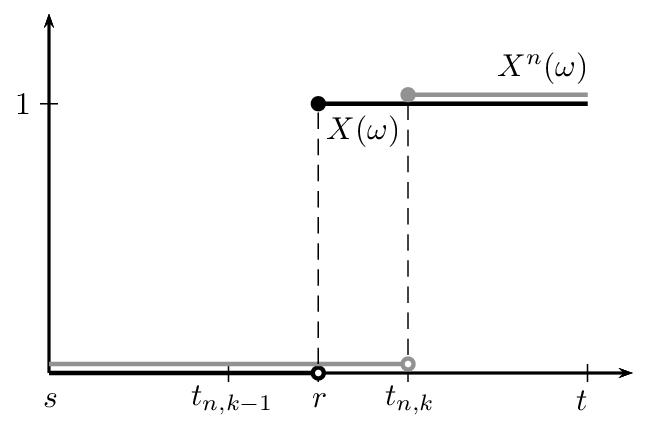
\includegraphics[scale =0.4] {obr1.jpg} %scale =0.4
   \label{skorochod1}
 }
 \subfigure[Time transformation]{
   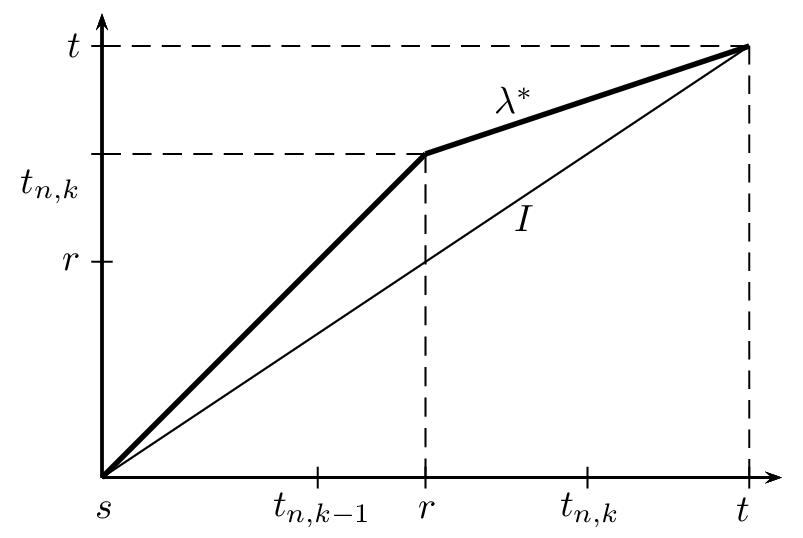
\includegraphics[scale =0.32] {obr2.jpg} %scale =0.32
   \label{skorochod2}
 }
\label{skorochod}
\caption{Reasoning for $X^n(\omega)\circ\lambda^*=X(\omega)$}
\end{figure}

For almost every  $\omega\in\Omega$ trajectory $X(\omega)$ has only finite number jumps in the interval $[s,t]$. Choose one such $\omega$. Because the state space is finite, size of each jump is finite. For clarity we will consider a trajectory $X(\omega)$ with only one jump of unit size. The general case with finite number of jumps is left as an exercise for the reader. So assume that $X(\omega)$ is of the form 
\[X(\omega,v)=\begin{cases}
0 & \text{if $v\in[s,r)$}\\ 
1 & \text{if $v\in[r,t]$}.
\end{cases}\]

For every partition $\Delta_n$ there exists $k$ for which $r\in(t_{n,k-1},t_{n,k}]$. 
As we can see from Figure \ref{skorochod1} the only difference between trajectories  $X^n(\omega)$ and $X(\omega)$ is that $X^n(\omega)$ is shifted right by $\sm{t_{n,k}-r}$. If we speed up the time appropriately on the interval $[0,r]$, the trajectory $X^n(\omega)$ would be equal to $X(\omega)$. Appropriate time transformation $\lambda^*\in\Lambda$ could be piecewise linear on intervals $[s,r]$, $[r,t]$ satisfying $\lambda^*(r)=t_{n,k}$. The function is plotted on Figure \ref{skorochod2}. Then evidently $X^n(\omega)\circ\lambda^*=X(\omega)$ and thus
\[\rho(X(\omega),X^n(\omega))\leq  \left\|\lambda^*-I\right\| \vee \left\|X(\omega)-X^n(\omega)\circ\lambda^*\right\| =\left\|\lambda^*-I\right\|\leq \left\|\Delta_n\right\|.\]
The result follows from the fact that the norm of the partition $\Delta_n$ goes to zero as $n$ goes to infinity.
\end{proof}
Like at the end of the previous section Section 1.2, define the matrix $\bm{\widetilde{R}}$ with entries $\widetilde{r}_{ij}=r_{i}$. When we replace the process $X$ by process the $X^n$ in equation \eqref{eqFactor}, we can express the second factor on the right hand side  as
\begin{equation}
\label{longterm}
\begin{split}
\mathbb{E}[-U_{s,t}^n(\bm{b})|\mathcal{F}_s]&\aseq\mathbb{E}\Big[-\mathcal{U}_{\gamma}^{\texttt{C}}\Big(\int_s^t r(X^n_v)\,dv + \sum_{s< v\leq t} r(X^n_{v-},X^n_{v})\Big)\cdot \bm{b}(X_t)\Big|\mathcal{F}_s\Big]\\
&\aseq\mathbb{E}\Big[-\mathcal{U}_{\gamma}^{\texttt{C}}\Big(\sum_{k=1}^n \tfrac{t-s}{n}\,r(X_{t_{n,k-1}})+\sum_{k=1}^n r(X_{t_{n,k}-},X_{t_{n,k}})  \Big)\cdot \bm{b}(X_t)\Big|\mathcal{F}_s\Big]\\
& \aseq \mathbb{E}\Big[ -\mathcal{U}_{\gamma}^{\texttt{C}}\Big(\sum_{k=1}^n \tfrac{t-s}{n} \widetilde{r}(X_{t_{n,k-1}},X_{t_{n,k}})+r(X_{t_{n,k-1}},X_{t_{n,k}})  \Big)\cdot \bm{b}(X_{t_{n,n}})\Big|\mathcal{F}_s\Big].
\end{split}
\end{equation}
Using Lemma \ref{LemmaSum} we can further simplify this term.
\begin{equation}
\label{longterm2}
\begin{split}
\mathbb{E}[-U_{s,t}^n(\bm{b})|\mathcal{F}_s]&\aseq \Big(\Big[\bm{P}_{\frac{t-s}{n}}\ast\bm{\exp}\{\gamma\,\tfrac{t-s}{n}\,\bm{\widetilde{R}}\} \ast\bm{\exp}\{\gamma\,\bm{R}\}\Big]^n\,\bm{b} \Big) (X_s)\\
&=\Big(\Big[\big(\exp\{\tfrac{t-s}{n}\,\gamma\,\diag(\bm{r})\}\cdot \exp\{\tfrac{t-s}{n}\,\bm{Q}\}\big) \ast\bm{\exp}\{\gamma\,\bm{R}\}\Big]^n\,\bm{b} \Big) (X_s).
%&=\Big(\Big[\exp\{\tfrac{t-s}{n}\,(\bm{Q}-\gamma\,\text{diag}(\bm{r}))\}\circ\bm{\exp}\{-\gamma\,\bm{R}\}\Big]^n\,\bm{b} \Big) (X_s)
\end{split}
\end{equation}
Using the Taylor expansion, it can be shown that last term converges to a finite limit. In spite of the simplicity of idea behind the proof, the proof itself is quite technical and tedious. Thus we move this computation to Appendix C. Now we can make the following conclusion.
%Accoring to the Proposition \ref{MatrixResult} the last term converges to a finite limit. 
\begin{prop}
\label{propC}
Let $0\leq s\leq s+h$. Then for any given vector $\bm{b}\in\mathbb{R}^N$ and the variable $U_{s+h}(\bm{b})$ defined by \eqref{UdefC} we have
$$\mathbb{E}[U_{s+h}(\bm{b})|\mathcal{F}_{s}]=U_{s}(\bm{S}^{h}\,\bm{b}),$$
where $\bm{S}^h$ has non-negative entries and is of the form
\begin{equation}
\label{SdefC}
\bm{S}^h=\exp\{h\,\bm{T}\}, \quad h\geq 0,
\end{equation}
where
\begin{equation}
\label{TdefC}
\bm{T}=(\bm{Q}+\gamma\,\diag(\bm{r}))\ast\bm{\exp}\{\gamma\,\bm{R}\}.
\end{equation}
\end{prop}
\begin{proof}
Define the functional $f$ on $D[s,t]$ by %\rightarrow\mathbb{R}
\[f(y)=-\mathcal{U}_{\gamma}^{\texttt{C}}\Big(\int_s^{s+h} r(y_v)\,dv + \sum_{s< v\leq s+h} r(y_{v-},y_{v})\Big)\cdot \bm{b}(y_t).\]
Because $f$ is continuous, according to Lemma \ref{Skorochod} $f(X^n)$ converges to the $f(X)$ almost surely. Moreover the sequence $f(X^n)$ is uniformly bounded, because the state space is finite. Thus we also have convergence in $L^1$ which implies convergence of conditional expectations. Now we can complete computation \eqref{longterm2} by taking the limit. The matrix $\bm{R}$ has zeros on its main diagonal. So according to the Lemma \ref{MatrixResult}
\begin{equation*}
\begin{split}
\lim_{n\rightarrow\infty}\Big[\exp\{\tfrac{h}{n}\,\gamma\,\diag&(\bm{r})\}\cdot \exp\{\tfrac{h}{n}\,\bm{Q}\} \ast\bm{\exp}\{\gamma\,\bm{R}\}\Big]^n\\
&=\exp\{(h)(\bm{Q}+\gamma\diag(\bm{r}))\ast\bm{\exp}\{\gamma\bm{R}\}\}=\bm{S}^{h}.\\
%&=\bm{S}^{t-s}
\end{split}
\end{equation*}
%Only non-negativity of $\bm{S}^h$ remains to be shown. This follows from the fact that 
The left hand side of the above term can be also expressed as %has non-negative entries because it can be expressed as... term  According to \eqref{longterm2} the matrix $\bm{S}^h$ can be also expressed as
$$\lim_{n\rightarrow\infty}\Big[\bm{P}_{\frac{h}{n}}\ast\bm{\exp}\{\gamma\,\tfrac{h}{n}\,\bm{\widetilde{R}}\} \ast\bm{\exp}\{\gamma\,\bm{R}\}\Big]^n.$$
So $\bm{S}^h$, $h\geq0$ is a limit of non-negative matrices and thus it is itself non-negative.
\end{proof}

%\begin{align*}
%\mathbb{E}\Big[&-u\Big(\sum_{k=1}^n \tfrac{t-s}{n}\,r(X_k^{s,t,n})+\sum_{k=1}^n r(X_{k-1}^{s,t,n},X_k^{s,t,n})  \Big)\cdot \bm{b}(X_t)\Big|\mathcal{F}_s\Big]\\
%& = \mathbb{E}\Big[ -u\Big(\sum_{k=1}^n \tfrac{t-s}{n} \widetilde{r}(X_{k-1}^{s,t,n},X_k^{s,t,n})+r(X_{k-1}^{s,t,n},X_k^{s,t,n})  \Big)\cdot \bm{b}(X^{s,t,n}_0)\Big|\mathcal{F}_s\Big]\\
%&= \Big(\Big[\bm{P}_{\frac{t-s}{n}}\circ\bm{\exp}\{-\gamma\,\tfrac{t-s}{n}\,\bm{\widetilde{R}}\} \circ\bm{\exp}\{-\gamma\,\bm{R}\}\Big]^n\,\bm{b} \Big) (X_s)\\
%&=\Big(\Big[\bm{P}_{\frac{t-s}{n}}\cdot\exp\{-\tfrac{t-s}{n}\,\gamma\,\text{diag}(\bm{r})\} \circ\bm{\exp}\{-\gamma\,\bm{R}\}\Big]^n\,\bm{b} \Big) (X_s)\\
%&=\Big(\Big[\exp\{\tfrac{t-s}{n}\,(\bm{Q}-\gamma\,\text{diag}(\bm{r}))\}\circ\bm{\exp}\{-\gamma\,\bm{R}\}\Big]^n\,\bm{b} \Big) (X_s).
%\end{align*}
%\begin{align}
%\Big[\bm{P}_{\frac{t-s}{n}}\circ\bm{\exp}\{-\gamma\,\bm{\widetilde{R}}\} \circ\bm{\exp}\{-\gamma\,\bm{R}\}\Big]^n&=\Big[\bm{P}_{\frac{t-s}{n}}\cdot\exp\{-\tfrac{t-s}{n}\,\gamma\,\text{diag}(\bm{r})\} \circ\bm{\exp}\{-\gamma\,\bm{R}\}\Big]^n\\
%&=\Big[\exp\{\tfrac{t-s}{n}\,(\bm{Q}-\gamma\,\text{diag}(\bm{r}))\}\circ\bm{\exp}\{-\gamma\,\bm{R}\}\Big]^n
%&=\exp\{(t-s)\,(\bm{Q}-\gamma\,\text{diag}(\bm{r}))\}\circ\bm{\exp}\{-\gamma\,\bm{R}\}
%\Big[\bm{P}_{\frac{t-s}{n}}\cdot\exp\{-\tfrac{t-s}{n}\,\gamma\,\text{diag}(\bm{r})\} \circ\bm{\exp}\{-\gamma\,\bm{R}\}\Big]^n%\exp\Big\{\tfrac{t-s}{n}\,\Big(\bm{Q}-\gamma\,\text{diag}(\bm{r})\Big)\Big\} \circ\bm{\exp}\{-\gamma\,\bm{R}\}\Big]^n
%&\longrightarrow \exp\Big\{(t-s)\,\Big(\bm{Q}-\gamma\,\text{diag}\{r_i\}_{i=1}^n\Big)\Big\} \circ\bm{\exp}\{-\gamma\,\bm{R}\}\Big\,\bm{b}(X_s)
%\end{align}
%It turns out that the last term converges to a finite limit. We can make the following conclusion.
%Denote $\bm{A}=\bm{Q}-\gamma\,\text{diag}(\bm{r})$ and $\bm{B}=\bm{\exp}\{-\gamma\,\bm{R}\}$. Than, because the matrix $\bm{R}$ has zeros on its main diagonal, $b_{ii}=1$ and according to Proposition \ref{MatrixResult} the last term converges to $\exp\{(t-s)\bm{A}\circ\bm{B}\}$. 
%\newpage
%$$r'(i,j)=\tfrac{t-s}{n}r(j)$$
%\begin{align}
%\mathbb{E}\Big[u\Big(\sum_{k=1}^n \tfrac{t-s}{n}\,r(X_k^{s,t,n}) \Big)\cdot b(X_t)\Big|\mathcal{F}_s\Big]&=
%[\bm{P}_{\frac{t-s}{n}}\circ\bm{\exp}\{-\gamma\,\bm{R}\}]^{n}\,b(X_s)\\
%&=\exp\Big\{\tfrac{t-s}{n}\,\bm{Q}\Big\}\,\exp\Big\{\tfrac{t-s}{n}\,\gamma\,\text{diag}\{r_1,\dots,r_N\}\Big\}\\
%&=\exp\Big\{\tfrac{t-s}{n}\,\Big(\bm{Q}-\gamma\,\text{diag}\{r_1,\dots,r_N\}\Big)\Big\}
%\end{align}
\vspace{2 mm}
%%%%%%%%%%%%%%%%%%%%%%%%%%%%%%%%%%%%%%%%%%%%%%%%%%%%%%%%%%%%%%%%%%%%%%%%%%%%%%%%%%%%%%%%%
\section{Optimal risk sensitive control of continuous time Markov decision chain}
\vspace{4 mm}

Similarly to the discrete time set-up, also here we add decisions to the process. Consider an action space
\[\mathcal{A}=\prod_{x\in\mathcal{X}}A_x,\]
 with $A_x$ representing the set of all admissible action in state $x$. For any policy $a\in\mathcal{A}$ let $\bm{Q}^a$ be an intensity matrix and $\bm{R}^a, \bm{r}^a$ be a reward matrix and a reward vector corresponding to the policy $a$. That is for every policy $a\in\mathcal{A}$ we have a continuous time Markov reward chain $X^a$.
 The whole system $(\Omega,\{\mathcal{F}_n\}_{n\in\mathbb{N}_0},\{$X$^a\}_{a\in\mathcal{A}})$ is called {\em a continuous time Markov decision chain}.

Consider a Markov decision chain with state space $\mathcal{X}=\{1,\dots,N\}$, intensity matrices
\[\bm{Q}^a=(\bm{q}_1(a_1),\dots,\bm{q}_N(a_N))\tr,\] 
reward matrices and reward vectors
\[\bm{R}^a=(\bm{r}_1(a_1),\dots,\bm{r}_N(a_N))\tr,\quad \bm{r}^a=(r_1(a_1),\dots,r_N(a_N))\tr.\] 
We assume that for all policies $a\in\mathcal{A}$ the chain is aperiodic and irreducibile. 
For any policy $a$ we have the variable $U_n^a(\cdot)$ defined by \eqref{UdefC} and the non-negative matrix  $\bm{S}^{a}=\exp\{\bm{T}^a\}$ defined by \eqref{SdefC} and \eqref{TdefC}. That is
\begin{align*}
\bm{T}^a=(\bm{t}_1(a_1),\dots,\bm{t}_N(a_N))\tr, \quad \bm{t}_i(a_i)&=\{t_{ij}(a_i)\}_{j=1}^{N},\\
 t_{ij}(a_i)&=(q_{ij}(a_i)+\gamma\,\delta_{ij}\,r_i(a_i)) \,e^{\gamma r_{ij}(a_i)},
\end{align*}
where $\delta_{ij}$ is the Kronecker delta. By virtue of the Perron-Frobenius theorem \ref{PF} the matrix $\bm{S}^a$ has its maximal eigenvalue $\lambda^a>0$ and respective eigenvector $\bm{v}^{a}>0$. In addition, according to the results of Appendix B, $\bm{v}^{a}$ is also an eigenvector of $\bm{T}^a$ coressponding to its maximal eigenvalue $\kappa^a\triangleq\log\lambda^a$.
%Consider a continuous time Markov decision chain with state space $\mathcal{X}=\{1,\dots,N\}$ such that for all policies $a\in\mathcal{A}$ the chain is aperiodic and irreducibile. For any fixed policy $a$ we have the nonnegative matrix $\bm{S}^a=\exp\{\bm{T}^a\}$ defined by \eqref{SdefC} and the variable $U_{t}^a(\cdot)$ defined by \eqref{UdefC}. 

%For a given $\widehat{a}\in\mathcal{A}$ denote $\widehat{\lambda}=\lambda^{\widehat{a}}$ and $\widehat{\bm{v}}=\bm{v}^{\widehat{a}}$. 
%$\exp\{u\widetilde{\bm{T}}\}=e^{-u\,\kappa}\,\bm{S}^{u}$
For fixed any $a\in\mathcal{A}$ consider a process
\begin{equation}
%\label{Mdef} 
M_{t}^{a}=(\lambda^a)^{-t}U_t^a(\bm{v}^a) \quad t\geq0.
\end{equation}
\begin{prop}
\label{MMlem}
The process $M_{t}^{a}$ is a $\mathcal{F}_t$-supermartingale if $\bm{T}^a\,\bm{v}^a\geq\kappa^a\,\bm{v}^a$. The process $M_{t}^{a}$ is a $\mathcal{F}_t$-martingale if $\bm{T}^a\,\bm{v}^a=\kappa^a\,\bm{v}^a$.
\end{prop}
\begin{proof}
As the Proposition concerns only one fixed policy, we will omit the upper index $a$ throughout the proof. %Denote $\kappa\triangleq\log\lambda$. 
First we want to show that the assumption $\bm{T}\,\bm{v}=\kappa\,\bm{v}$ implies the inequality  \[\exp\{s\,\bm{T}\}\,\bm{v}=\bm{S}^s\,\bm{v}\geq\lambda^s\,\bm{v}=e^{s\,\kappa}\,\bm{v} \quad\text{for all } s\geq0.\]
Using the fact $\exp\{-s\kappa\,\bm{I}\}=e^{-sk}\bm\,\bm{I}$ we compute
\begin{align*}
\bm{S}^s\,\bm{v}-\lambda^s\,\bm{v}&=\exp\{s\,\bm{T}\}\,\bm{v}-e^{s\,\kappa}\,\bm{v}\\
&=e^{s\,\kappa}\,(e^{-s\,\kappa}\,\exp\{s\,\bm{T}\}\,\bm{v}-\bm{v})\\
&=e^{s\,\kappa}\,(\exp\{s(\underbrace{\bm{T}-\kappa\,\bm{I}}_{\triangleq\widetilde{T}})\}-\bm{I})\,\bm{v}.
\end{align*}
The last equality is true due to the fact that matrices $\bm{T}$ and $\kappa\,\bm{I}$ commute. Denote $\widetilde{\bm{T}}\triangleq \bm{T}-\kappa\,\bm{I}$. Then by assumption $\widetilde{\bm{T}}\,\bm{v}\geq0$. We continue with computation as follows
\begin{align*}
\bm{S}^s\,\bm{v}-\lambda^s\,\bm{v}&=e^{s\,\kappa}\,(\exp\{s\widetilde{\bm{T}}\}-\bm{I})\,\bm{v}\\
&=e^{s\,\kappa}\,\left(\int_0^s \frac{\mathrm{d}}{\mathrm{d}u}\exp\{u\widetilde{\bm{T}}\}\mathrm{d} u \right)\,\bm{v}
=\underbrace{e^{s\,\kappa}}_{\geq 0}\,\left(\int_0^s \exp\{u\widetilde{\bm{T}}\}\mathrm{d} u\right) \,\underbrace{(\widetilde{\bm{T}}\bm{v})}_{\geq 0}.
\end{align*}
The integrant $\exp\{u\widetilde{\bm{T}}\}=e^{-u\,\kappa}\,\bm{S}^{u}$ is also non-negative according to Proposition \ref{propC}. Thus the whole term is nonnegative. 

We have shown that $\bm{S}^s\,\bm{v}\geq\lambda^s\,\bm{v}$, $s\geq0$. Employing  the Proposition \ref{propC} and the fact that $M_{s}$ is $\mathcal{F}_{s}$ measurable we get
\begin{align*}
\mathbb{E}[M_{s+h}-M_{s}|\mathcal{F}_{s}]&=\lambda^{-(s+h)}\,U_{s}(\bm{S}^h \bm{v}) - \lambda^{-s}\,U_{s}(\bm{v})\\
&=\lambda^{-s-h}[U_{s}(\bm{S}^h\bm{v})-\lambda^h\,U_{s}(\bm{v})]\\
&=\underbrace{\lambda^{-s-h}}_{> 0}\,\underbrace{U_{s}}_{< 0}\cdot[(\bm{S}^h\,\bm{v})(X_{s})-(\lambda^s\,\bm{v})(X_{s})].
\end{align*}
Because $\lambda$ is positive and $U_{s}$ is negative we have 
\[ \lambda^s\,\bm{v} \leq \bm{S}^s\,\widehat{\bm{v}} \quad \Longrightarrow \quad \mathbb{E}[M_{s+h}|\mathcal{F}_{s}]\asleq M_{s}, \quad 0\leq s \leq s+h. \qedhere\]
\end{proof}

\begin{thm}
If the inequality $\bm{T}^a\,\bm{v}^{\widehat{a}}\geq\kappa^{\widehat{a}}\,\bm{v}^{\widehat{a}}$ holds for every policy $a\in\mathcal{A}$, then $\widehat{a}$ is an optimal policy.
%If $M_{n}^{a}$ is a supermartingale for all $a\in\mathcal{A}$, than $\widehat{a}$ is an optimal policy.
\end{thm}
\begin{proof}
In the proof of the Lemma \ref{MMlem} we show that the assumption implies  
\[\bm{S}^a\,\bm{v}^{\widehat{a}}\geq\lambda^{\widehat{a}}\,\bm{v}^{\widehat{a}} \quad \text{for all  $a\in\mathcal{A}$.}\]
The rest is a direct analogue of the proof of the Theorem \ref{criteria}.
\end{proof}
\begin{thm}[Policy iteration]
\label{PolicyIiterationC}
Let $a_{0}\in\mathcal{A}$ be the initial policy. Let $a_{0}\in\mathcal{A}$ be the initial policy. Define sequence $\{a_n\}$ recursively by 
\begin{equation}
\label{minimizationC}
%a_{n+1}=\underset{a\in\mathcal{A}}{\operatorname{argmin}}\,\bm{S}^{a}\bm{v}^{a_n}
a_{n+1}(i)=\underset{a\in\mathcal{A}}{\operatorname{argmin}}\,\bm{t}^a_i\,\bm{v}^{a_n}.
\end{equation}
If the minimum is attained for more the one policy and $a_n$ is one of then, always make conservative choice $a_{n+1}(i)=a_{n}(i)$. Then $a_n$ converges to an optimal policy $\widehat{a}$.
\end{thm}
\begin{proof} 
%According to ?? the maximal eigenvector of $\bm{T}^a$ is equal to $\kappa^a=\log(\lambda^a)$. Moreover $\bm{v}^{a}$ is eigenvector corresponding to $\kappa^a$. 
Suppose that $a_n$ converges to $\widehat{a}$. Then by \eqref{minimizationC} for all $i$ we have
\begin{equation*}
\label{problemeq}
\bm{e}_i\tr\,\bm{T}^a\,\bm{v}^{\widehat{a}}\geq \bm{e}_i\tr\,\bm{T}^{\widehat{a}}\,\bm{v}^{\widehat{a}}=\kappa^{\widehat{a}}\,v_i^{\widehat{a}} \quad a\in\mathcal{A}
\end{equation*}
Thus the inequality $\bm{T}^a\,\bm{v}^{\widehat{a}}\geq\kappa^{\widehat{a}}\,\bm{v}^{\widehat{a}}$ holds for every $a\in\mathcal{A}$ and the policy $\widehat{a}$ is optimal by virtue of Theorem \ref{criteria2}. %In \eqref{problemeq} we use that $\bm{v}^a$ is an eigenvector of $\bm{T}^a$ corresponding to its eigenvalue  $\log(\lambda^a)$  {(\color{red}!!! Je potrebne formulovat nejake lemma bez dukazu ze toto plati?)} 
The rest is a direct analogue of the proof of the Theorem \ref{PolicyIteration}.
\end{proof}

The Theorem \ref{PolicyIiterationC} gives us a method for finding the optimal policy for continuous time Markov Chain. The algorithm works exactly as for discrete time case, which is described at the end of section 1.3. The only difference is that the matrix $\bm{S}$ is replaced by the matrix $\bm{T}$, which is given by \eqref{TdefC}.

%\newpage


